
\section{Тест производительности}

Для тестов я использвал утилиту gnuplot для построения графиков зависимости времени работы программы от величины числа. Так же для сравнения использовал библиотеку chrono для замера времени.

\begin{figure}[h]
  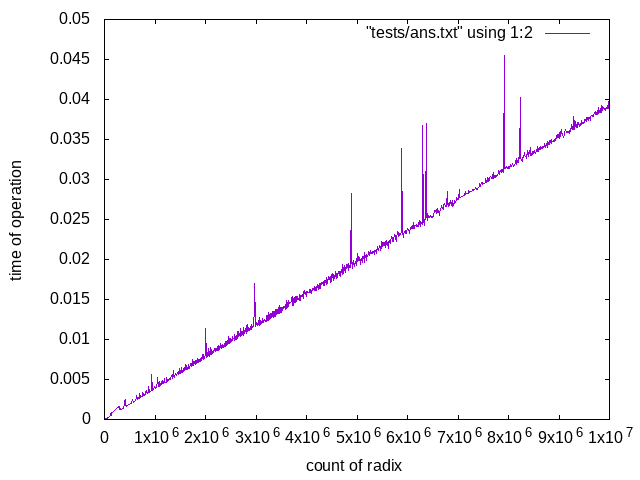
\includegraphics[scale=0.5]{../plots/dpversionwithoutway.png}
  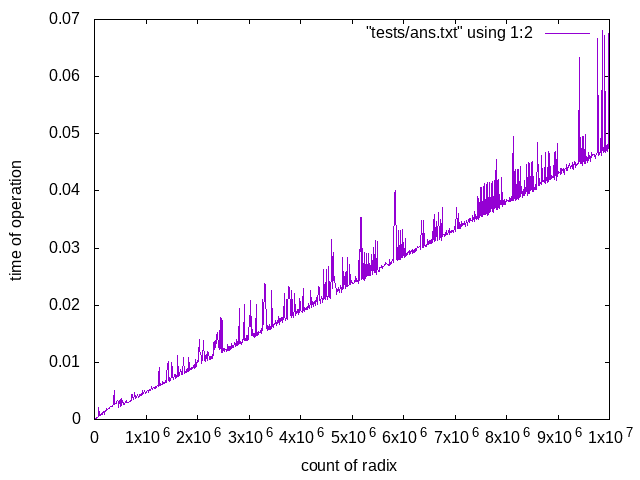
\includegraphics[scale=0.5]{../plots/dpversion.png}
  \caption{Графики работы с поиском пути и без него}
\end{figure}

\begin{figure}[h]
  \begin{center}
    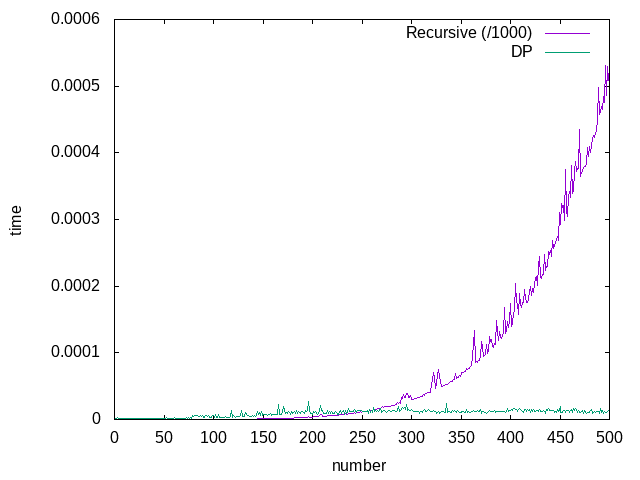
\includegraphics[scale=0.7]{../plots/dpandnot.png}
  \end{center}
  \caption{Графики работы наивного алгоритма и с приминением методов динамического программирования}
\end{figure}

\pagebreak
